\documentclass[10pt,a4paper,twocolumn]{article}

\usepackage[T1]{fontenc}
\usepackage[utf8]{inputenc}
\usepackage{mathptmx}
\usepackage[scaled=0.9]{helvet}
\usepackage[a4paper,margin=1.8cm,columnsep=0.7cm]{geometry}
\usepackage{microtype}
\usepackage{xcolor}
\usepackage{tikz}
\usetikzlibrary{arrows.meta,positioning,calc}
\usepackage{enumitem}
\usepackage{titlesec}
\usepackage{caption}
\usepackage{stfloats}
\usepackage[hidelinks]{hyperref}

\definecolor{model}{HTML}{3B3486}
\definecolor{modelline}{HTML}{6C63C7}
\definecolor{code}{HTML}{E9E7E1}
\definecolor{codeline}{HTML}{8A877E}
\definecolor{ink}{HTML}{1C1B19}
\definecolor{wire}{HTML}{6F6C64}

\setlist{nosep,leftmargin=1.2em}
\titleformat{\section}{\normalsize\bfseries}{\thesection}{0.6em}{}
\titlespacing*{\section}{0pt}{0.9em}{0.3em}
\titleformat{\paragraph}[runin]{\normalsize\itshape}{}{0pt}{}[.]
\titlespacing*{\paragraph}{0pt}{0.45em}{0.5em}
\captionsetup{font=small,labelfont=bf}
\setlength{\textfloatsep}{1.0em}
\newcommand{\lbl}[2]{\textbf{#1}\\[-1pt]{\footnotesize #2}}
\newcommand{\C}{\ensuremath{C}}

\title{\vspace{-1.4cm}\textbf{ProcureCabana: A Procurement Agent\\
that Optimises Beyond Unit Price}\vspace{-0.3em}}
\author{Team Codacabana\\[0.1em]
{\small Tacto Negotiation Arena, EHL Grand Finale, Munich, October 2026}}
\date{}

\begin{document}

\twocolumn[
\maketitle
\vspace{-2.2em}
\begin{center}
\begin{minipage}{0.88\textwidth}
\small
\textbf{Abstract.}
We describe ProcureCabana, an autonomous procurement agent that negotiates by e-mail with simulated suppliers
and concludes each case with either a single accepted term sheet or a withdrawal. Performance is
measured on total cost \C{} over the case horizon rather than on unit price; the agent therefore
optimises payment terms, delivery, contract duration, quality provisions and index clauses
jointly with price. The architecture separates two responsibilities. Deterministic code computes
every binding quantity and verifies it against the arena's cost function. A team of
language-model subagents analyses the supplier, rehearses the negotiation and composes the
correspondence, and its output is constrained by code before use. On the ten hosted practice
cases the agent concluded ten agreements with a mean score of 0.777.
\end{minipage}
\end{center}
\vspace{0.4em}
]

\begin{figure*}[b]
\centering
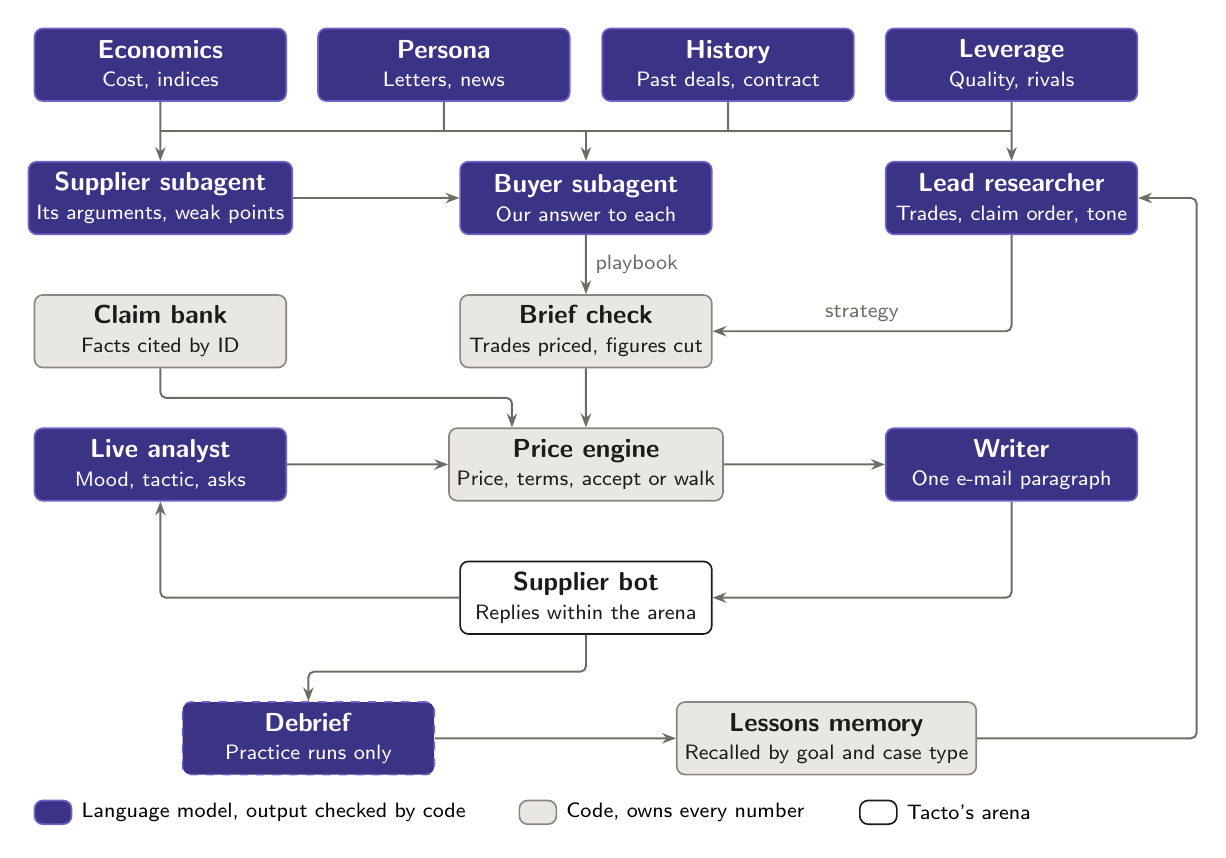
\begin{tikzpicture}[scale=0.94, transform shape,
  font=\sffamily,
  box/.style={rounded corners=3pt, minimum width=3.4cm, minimum height=0.98cm, align=center,
              inner sep=3pt, line width=0.6pt},
  model/.style={box, fill=model, draw=modelline, text=white},
  code/.style={box, fill=code, draw=codeline, text=ink},
  arena/.style={box, fill=white, draw=ink, text=ink},
  wire/.style={draw=wire, line width=0.7pt, -{Stealth[length=5pt]}, rounded corners=2pt},
  bus/.style={draw=wire, line width=0.7pt},
]

% specialists
\node[model] (eco) at (0.5,0)   {\lbl{Economics}{Cost, indices}};
\node[model] (per) at (4.33,0)  {\lbl{Persona}{Letters, news}};
\node[model] (his) at (8.17,0)  {\lbl{History}{Past deals, contract}};
\node[model] (lev) at (12,0)    {\lbl{Leverage}{Quality, rivals}};

% rehearsal and lead
\node[model] (sup)  at (0.5,-1.8)  {\lbl{Supplier subagent}{Its arguments, weak points}};
\node[model] (buy)  at (6.25,-1.8) {\lbl{Buyer subagent}{Our answer to each}};
\node[model] (lead) at (12,-1.8)   {\lbl{Lead researcher}{Trades, claim order, tone}};

% code checks
\node[code] (bank)  at (0.5,-3.6)  {\lbl{Claim bank}{Facts cited by ID}};
\node[code] (brief) at (6.25,-3.6) {\lbl{Brief check}{Trades priced, figures cut}};

% live loop
\node[model] (ana) at (0.5,-5.4)  {\lbl{Live analyst}{Mood, tactic, asks}};
\node[code]  (eng) at (6.25,-5.4) {\lbl{Price engine}{Price, terms, accept or walk}};
\node[model] (wri) at (12,-5.4)   {\lbl{Writer}{One e-mail paragraph}};

\node[arena] (bot) at (6.25,-7.2) {\lbl{Supplier bot}{Replies within the arena}};

% after the case
\node[model, dashed] (deb) at (2.5,-9.1) {\lbl{Debrief}{Practice runs only}};
\node[code]  (mem) at (9.5,-9.1) {\lbl{Lessons memory}{Recalled by goal and case type}};

% specialists to the team
\draw[bus] (eco.south) -- (0.5,-0.9);
\draw[bus] (per.south) -- (4.33,-0.9);
\draw[bus] (his.south) -- (8.17,-0.9);
\draw[bus] (lev.south) -- (12,-0.9);
\draw[bus] (0.5,-0.9) -- (12,-0.9);
\draw[wire] (0.5,-0.9) -- (sup.north);
\draw[wire] (6.25,-0.9) -- (buy.north);
\draw[wire] (12,-0.9) -- (lead.north);

\draw[wire] (sup) -- (buy);
\draw[wire] (buy) -- node[right, font=\sffamily\footnotesize, text=wire] {playbook} (brief);
\draw[wire] (lead.south) |- node[pos=0.75, above, font=\sffamily\footnotesize, text=wire] {strategy} (brief.east);
\draw[wire] (brief) -- (eng);
\draw[wire] (bank.south) -- (0.5,-4.5) -| ([xshift=-1cm]eng.north);

\draw[wire] (ana) -- (eng);
\draw[wire] (eng) -- (wri);
\draw[wire] (wri.south) |- (bot.east);
\draw[wire] (bot.west) -| (ana.south);
\draw[wire] (bot.south) -- (6.25,-8.2) -| (deb.north);
\draw[wire] (deb) -- (mem);
\draw[wire] (mem.east) -- (14.5,-9.1) |- (lead.east);

% legend
\node[model, minimum width=0.5cm, minimum height=0.32cm] (l1) at (-0.95,-10.1) {};
\node[anchor=west, font=\sffamily\footnotesize] at (l1.east) {Language model, output checked by code};
\node[code, minimum width=0.5cm, minimum height=0.32cm] (l2) at (5.6,-10.1) {};
\node[anchor=west, font=\sffamily\footnotesize] at (l2.east) {Code, owns every number};
\node[arena, minimum width=0.5cm, minimum height=0.32cm] (l3) at (10.2,-10.1) {};
\node[anchor=west, font=\sffamily\footnotesize] at (l3.east) {Tacto's arena};
\end{tikzpicture}
\caption{System overview. The playbook additionally supplies the live analyst with the arguments
to recognise and the writer with the prepared response. The debrief is drawn dashed because the
final round returns no score; in that round the agent relies on the lessons recorded during
practice.}
\label{fig:system}
\end{figure*}

\section{Problem setting and design principle}

A case specifies the buyer's category goal, a set of mandatory requirements, the negotiable
fields with their admissible options, and one or more suppliers, each with an opening quotation.
The score of a case is $(C_\mathrm{open}-C_\mathrm{deal})/(C_\mathrm{open}-C_\mathrm{best})$.
The arena imposes a round limit per thread (ten buyer messages by default) and allows 60 seconds per reply, and the final round is
conducted without human intervention.

Language models interpret a counterpart's correspondence well, but their arithmetic cannot be
relied upon without verification. We therefore assign \emph{every binding quantity to code}:
prices, term sheets, acceptance and withdrawal are computed and verified with the arena's
published cost function and its check of the mandatory requirements. Models either select from
enumerated options or produce text that is subsequently filtered. Each model invocation is
subject to a timeout with a deterministic fallback, so that a move is issued within the reply deadline even when a model fails. Decisions are conditioned on the evidence available about a supplier and never on a
case or supplier identifier.

\section{Preparation}

Before a session is opened, and hence before any reply deadline applies, a research team is
allotted 40 seconds per case (Figure~\ref{fig:system}, top).

\paragraph{Specialists} Four subagents each examine one category of data and report at most four
findings together with an assessment of which party holds the leverage. \emph{Economics}
considers our should-cost estimate, the supplier's price history and the indices of its cost
drivers. \emph{Persona} considers the company profile, correspondence, meeting notes and news
coverage. \emph{History} considers previous negotiations and the contract with its clauses.
\emph{Leverage} considers delivery and quality performance, our demand forecast, our purchase
orders and competing quotations.

\paragraph{Lead researcher} The lead consolidates these findings, together with the outcomes of
comparable earlier cases, into a strategy comprising at most two term trades, the ordering of our
arguments and the tone of the correspondence. It determines neither prices nor the pace of
concession.

\paragraph{Rehearsal} A supplier subagent, acting in character, states the arguments it intends
to advance and the weaknesses it hopes will go unnoticed. A buyer subagent then responds to each
argument. The outcome is a playbook of anticipated arguments paired with prepared responses.

\paragraph{Validation} A proposed trade is admitted only if it is an admissible option of a
negotiable field, and any playbook line containing a digit is discarded. Where no data exist for a
supplier, all trades and weaknesses are removed, so that the agent asserts nothing that our
records do not support.

Concurrently, code derives a supplier profile from fixed textual patterns (liquidity need, spare or full capacity, frozen prices, hedged material), takes our should-cost as the estimate of the supplier's full cost, and infers its cost of capital from ownership type, liquidity need and cash discount. It also constructs a claim bank of statements, each
citing a record identifier and the corresponding figure. Every figure the agent cites is drawn from this bank.

\section{Offer policy}

\paragraph{Terms} Every admissible combination of non-price terms is evaluated at the supplier's
own valuation, and the combination yielding the lowest \C{} is retained. A term that is
inexpensive for the buyer yet valuable to the supplier, such as accelerated payment for a
supplier with a liquidity need, can thus be exchanged for a price reduction.

\paragraph{Opening} The opening price is a fraction of the quotation set by the category goal, from 0.78 in leverage cases to 0.92 in stabilisation cases, and raised for suppliers with frozen prices, full capacity or near-cost pricing. The trades proposed by
the lead are issued as additional term sheets, each priced so that its cost to the buyer equals
that of the principal sheet. The supplier's choice among them consequently reveals its
preferences at no cost to the buyer.

\paragraph{Subsequent rounds} In each round the agent closes 30\,\% of the gap to the supplier's
counter-offer. Following a large initial concession it holds its position, as such a concession
indicates a low reservation price. A patience budget limits the gaps presented under relationship-oriented goals and to suppliers priced near cost or operating at full capacity. A live analyst reads each reply in at most six seconds and returns a mood, one of three tactics and the anticipated argument it has
recognised: \emph{hold} reduces the step to 70\,\% of its usual size, whereas \emph{argue} adds
one further claim. Three claims accompany the first message and one each subsequent message.

\paragraph{Bounds} No term sheet exceeds the price at which \C{} equals the cost of the buyer's
alternative. Under relationship-oriented goals, where a full-cost estimate exists, the price is not reduced beyond the point at which the relationship charge causes \C{} to increase.

\paragraph{Correspondence} The writer model responds to the supplier's most recent message in a
single paragraph free of digits and identifiers. Code appends the figures, claims and term
sheets, and substitutes a template whenever the paragraph is late or rejected.

\section{Termination}

The agent concludes a case upon the supplier's final offer, upon its agreement, at the round
limit, or at least 90 seconds before the time limit of a wave. Only a standing term sheet is eligible for
acceptance. A sheet qualifies if it states a price, satisfies every mandatory requirement and
costs less than the buyer's alternative. Among several bidders, the qualifying sheet of lowest
cost is accepted. If no sheet qualifies, the agent withdraws. Where a supplier's final offer would be refused, the agent first submits one sheet at its price ceiling.

\section{Empirical observations on supplier behaviour}

The policy encodes observations drawn from our own sandbox and practice sessions. Most are
supported by one to three sessions per supplier and should be read accordingly.
\begin{itemize}
\item Suppliers conceded in response to a move on our part and agreed once our sheet reached the
  counter-offer they would otherwise make; an unchanged sheet drew no concession in the sandbox.
  Our sheet is therefore kept below their counter-offer until the close.
\item Verified claims that a supplier took into account lowered its counter-offers, mostly in the
  first round: one sandbox supplier countered at 51.30 without claims and at 50.00 with three.
  Claims a supplier judged irrelevant had no effect.
\item Final offers arrived at a cumulative gap of 36 to 42\,\% between our sheets and their
  counter-offers in four cases, and at 15 to 19\,\% for two less patient suppliers.
\item Bluffs and urgency left the price unchanged (three runs each), and all twelve suppliers
  asked declined to share a cost breakdown. The agent employs none of these.
\end{itemize}
After each practice case, code records the price trajectories and the score, and a debrief model
contributes one lesson, indexed by goal, case type, ownership type and observed traits. The lead
researcher is given the figures of the most similar earlier runs rather than the written lesson,
since a single run constitutes an observation and not a rule.

\section{Results and limitations}

One practice session per hosted case yielded ten agreements in ten cases and a mean score of
0.777. In that batch, 121 of 127 subagent invocations succeeded, and the six that timed out
reverted to the deterministic path. On the preceding evening the mean of our best scores per case was 0.776, third of 24 on the practice leaderboard.

Two limitations should be noted. First, a single batch does not constitute a paired comparison,
and we are unable to demonstrate that the subagent team outperforms the price engine alone.
Second, the full-cost estimate depends on a should-cost figure with a stated error of 5 to
15\,\%; the agent mitigates this by bounding the estimate with the supplier's own offers.

\end{document}
